\section{Segmentation using Unsupervised Methods}\label{secunsupervised}
In the beginning, established, unsupervised methods were used to segment the images in order to gain a better understanding of the data. Unsupervised learning includes algorithms which intend to find regularities, structures, or patterns within unlabelled datasets. As they require no ground truth labelled data and are not too computationally expensive, they are a great fit for exploratory analysis. The results of two classical methods (watershed and ellipse fitting) applied to the given images are discussed in the following. For this section, one myotube-myoblast image pair in Fig.~\ref{figtubeblast} and Fig.~\ref{figoverlap} will be used to exemplify the unsupervised methods. \texttt{OpenCV} \cite{opencv_library} was used exclusively for this entire section.
\begin{figure}
	\centering
	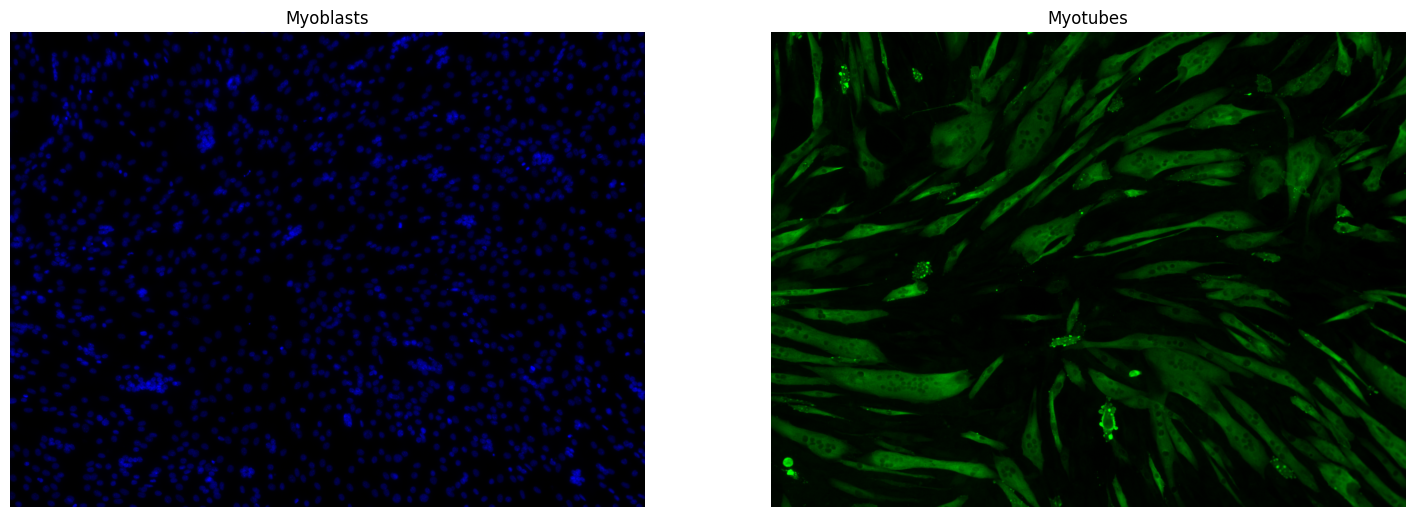
\includegraphics[width=\textwidth]{"images/workhorse.png"}
	\caption[Workhorse image of myoblasts and myotubes]{Microscopy image of myotubes and myoblasts. In this juxtaposition it is clearly visible that some myoblasts form the nuclei of the myotubes due to the dark circles within them.}
	\label{figtubeblast}
\end{figure}

\begin{figure}
	\centering
	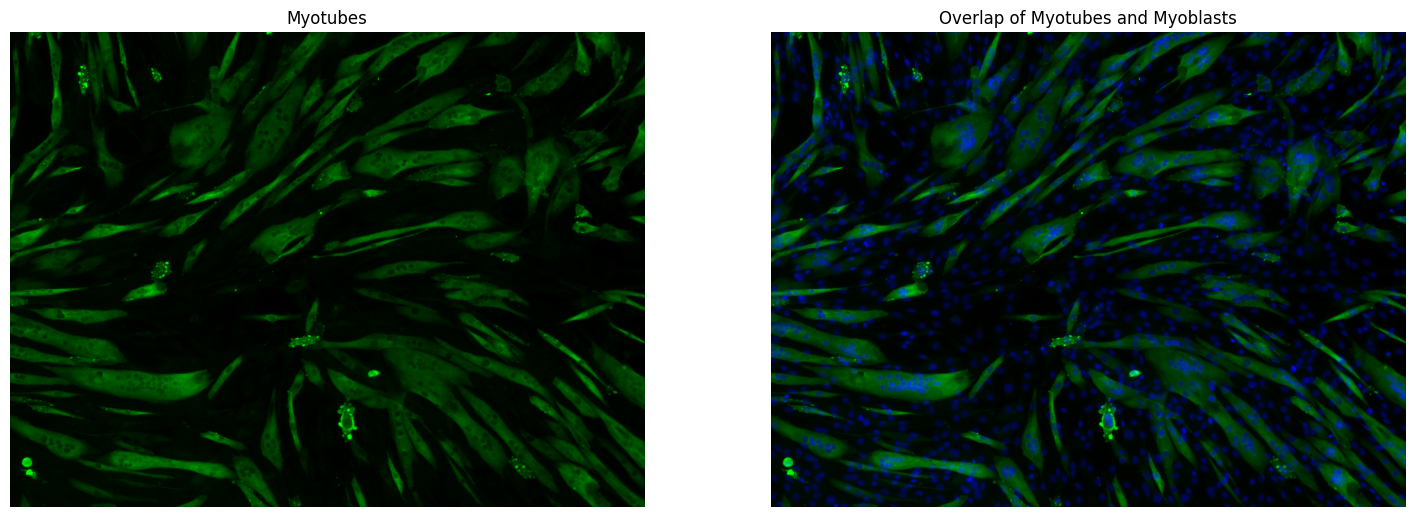
\includegraphics[width=\textwidth]{"images/overlap.png"}
	\caption[Overlap of myoblasts and myotubes]{Overlap of myoblasts and myotubes. It clearly shows what myoblasts have become nuclei to myotubes.}
	\label{figoverlap}
\end{figure}

\subsection{Exploratory Data Analysis}\label{secexploratory}
Myotube and cell nuclei microscopy images significantly differ from natural images. While cell nuclei images tend to be more homogeneous in size and shape of the nuclei, presenting replicable challenges, myotube images exhibit far greater diversity. Our exploratory data analysis aimed to understand the characteristics of myotube images, both quantitatively and qualitatively.

\subsubsection{Qualitative Analysis}
\begin{figure}
	\centering
	\includegraphics[width=\textwidth]{"images/myotube_image_set.png"}
	\caption[TBD]{\textcolor{red}{TBD}}
	\label{fig1}
\end{figure}
In the myotube image set eventually used for training, it is clear that these images vary widely in size, brightness, and color schemes. They are primarily monochromatic, with their color depending on the marker used to make the myotubes visible and the type of microscope employed for capturing the images. Additionally, the myotubes themselves display considerable variation in size, shape, and density. This variety underscores the diverse data distribution present within myotube images as a whole.

\subsubsection{Quantitative Analysis}
Upon evaluating the images selected for training, we found that myotube images are predominantly dark. The evaluated images had average red, green, and blue values of 2.56, 9.8, and 2.9, respectively, with a high degree of variance. Further analysis into the HSL (Hue, Saturation, Lightness) space of these images confirmed their darkness, primarily attributed to the large areas of dark background present. The figure below summarizes the activations for red, green, blue, and lightness across several images.

\begin{tabular}{|p{2cm}|p{2cm}|p{2cm}|p{2cm}|p{2cm}|p{2cm}|}
	\hline
	& Minimum Activation & Minimum non-zero  activation & Maximum activation & Mean of mean activations & Mean of activation standard deviations \\
	\hline
	Red & 0 & 1.89 & 6.90 & 2.56 & 3.88 \\
	\hline
	Green & 0 & 1.89 & 28.34 & 9.79 & 8.13 \\
	\hline
	Blue & 0 & 2.84 & 17.48 & 2.90 & 2.36 \\
	\hline
	Lightness & 0.64 & NA & 14.23 & 5.37 & 4.75 \\
	\hline
\end{tabular}

\begin{figure}
	\centering
	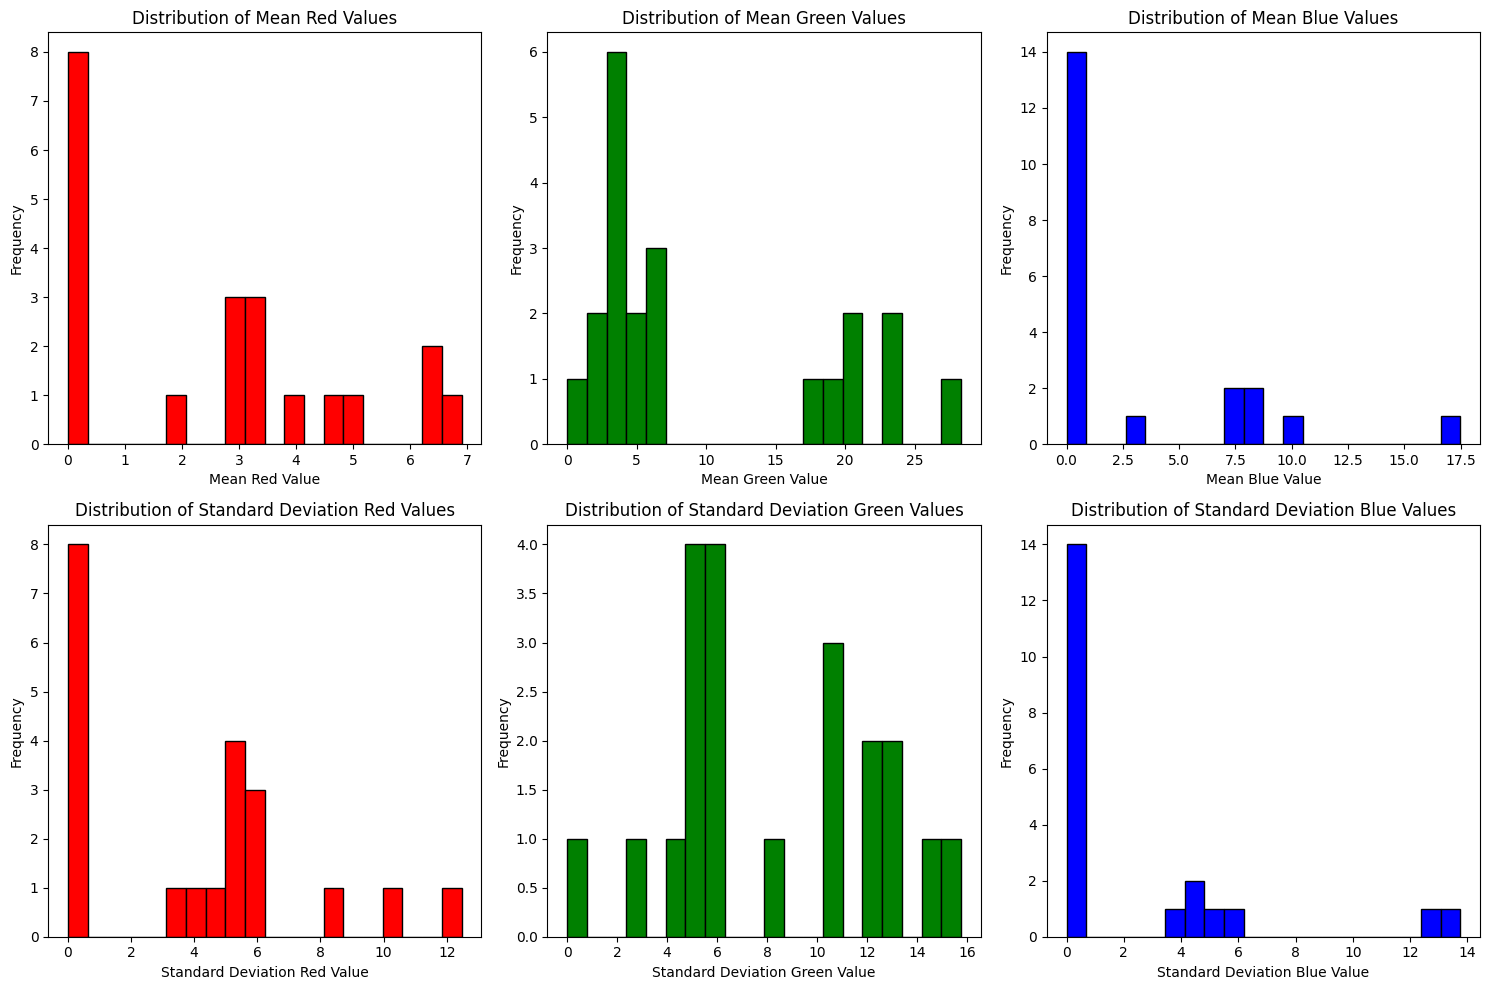
\includegraphics[width=\textwidth]{"images/pixel_distribution_plots_rgb.png"}
	\caption[TBD]{\textcolor{red}{TBD}}
	\label{fig2}
\end{figure}
\begin{figure}
	\centering
	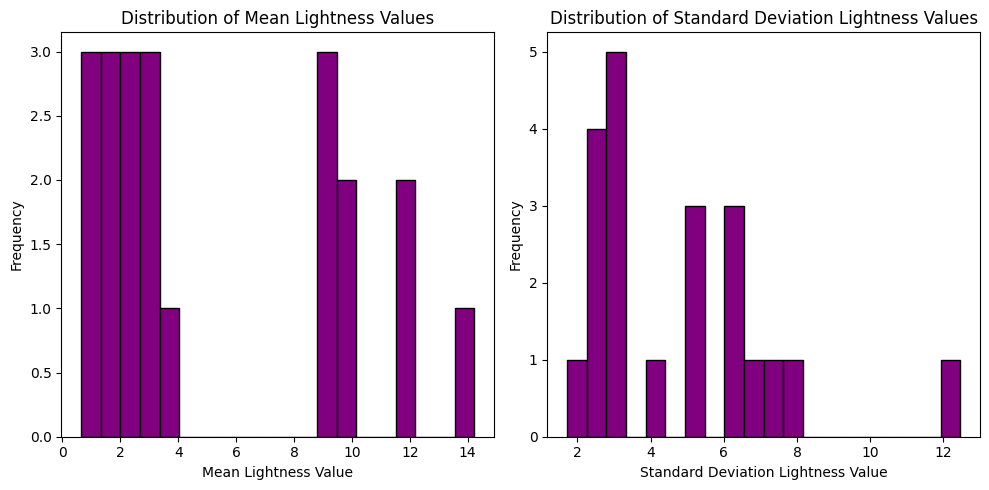
\includegraphics[width=\textwidth]{"images/pixel_distribution_plots_hsl.png"}
	\caption[TBD]{\textcolor{red}{TBD}}
	\label{fig3}
\end{figure}
\ \\
This analysis highlights the necessity of treating myotube images differently from natural images. For instance, typical normalization techniques based on pixel activation means derived from natural images are not directly applicable to myotube images due to their unique characteristics.

\subsection{k-Means Clustering and Otsu Thresholding}
As a starter, foreground detection algorithms were tried out in order to discriminate between cells, be it myotubes or myoblasts, and background. There are two common methods to do so in computer vision. 

The first one is the k-Means algorithm, whose goal it is to minimize the within-class-variance of a (predetermined) number of $k$ clusters \cite{bishop2006}. To this end, $k$ points are initialized and function as the first centers of the clusters. All observations are then grouped by proximity to the centers (according to some distance measure, commonly the $L2-$norm). This procedure is reiterated until convergence. In its simplest form, all initial points are drawn from a uniform distribution. A more common implementation is the k-Means++ algorithm \cite{kmeans} which samples only one point from a uniform distribution. All other points are sampled from a distribution proportional to the (squared) distance to the first point so as to minimize the chance of drawing cluster centers close to one another.

In order to use k-Means for image segmentation, the image first needs to be transformed to grayscale. Upon calculating the histogram of pixel intensities, the counts for every bin are the observations. Using $k = 2$ results in one threshold value seperating two intervals. All pixels with values above this threshold are considered foreground, all the other ones are background.

In a similar vein, Otsu's method \cite{otsu} was utilized. In many ways, Otsu thresholding is not too different from k-Means in the sense that it also minimizes within-class-variance of the grayscale histogram. They can even be shown to be equivalent but only the Otsu method guarantees convergence to the global optimum \cite{liu2009otsu}. Implementation wise, variance estimates are calculated explicitly by iterating the threshold over all possible grayscale values to find the optimal one with respect to the within-class variance as the objective function.

Both foreground detection algorithms applied to Fig.~\ref{figtubeblast} can be found in Fig.~\ref{figkmblast}-\ref{figotsutube}. While this is not instance segmentation per se and therefore one cannot distinguish between overlapping cell instances, it is very helpful to gain intuition on the available images. One major drawback of thresholding methods is the fact that a hard cutoff implies that instances that are too dim are taken to be background.
\begin{figure}
	\centering
	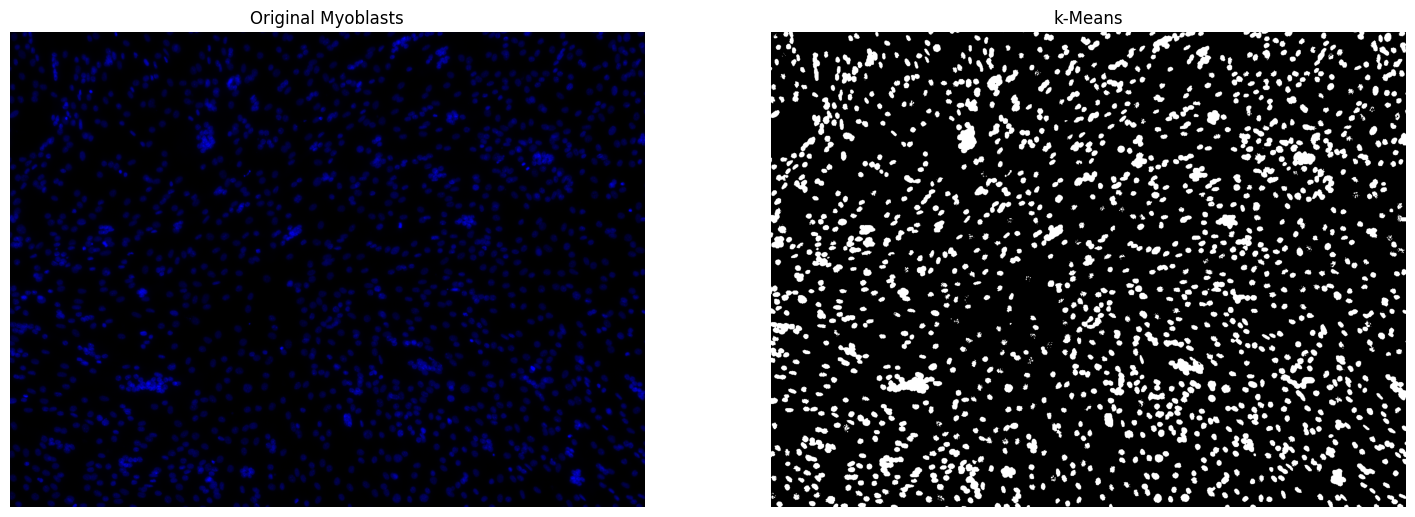
\includegraphics[width=\textwidth]{"images/km_blast.png"}
	\caption[k-Means applied to myoblasts]{Foreground detection of myoblasts using k-Means}
	\label{figkmblast}
\end{figure}
\begin{figure}
	\centering
	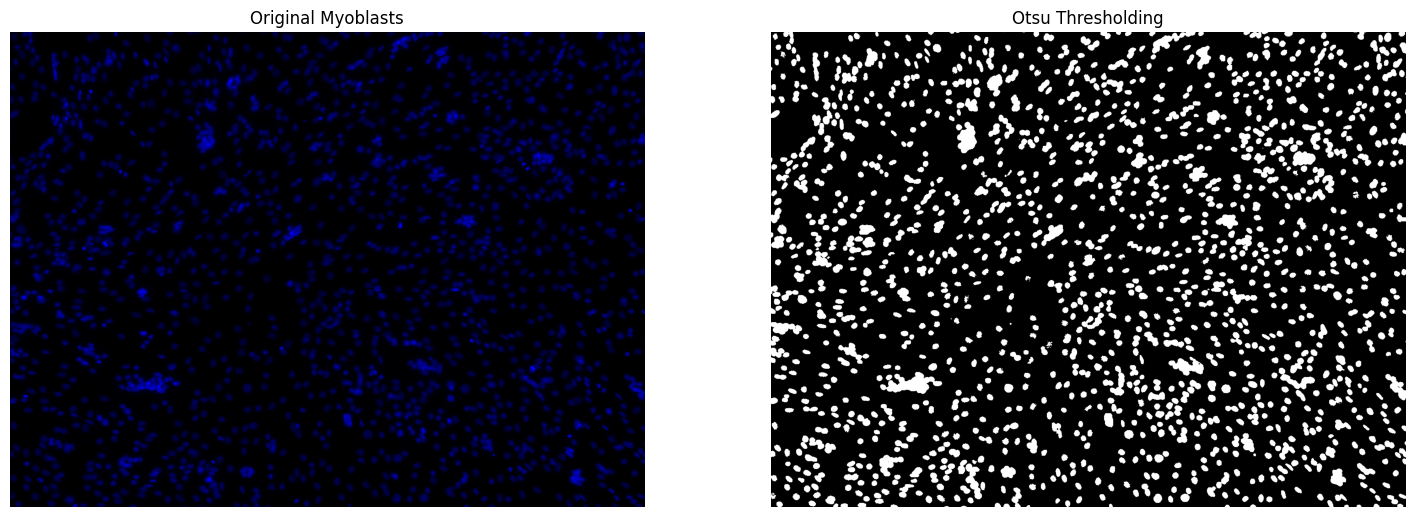
\includegraphics[width=\textwidth]{"images/otsu_blast.png"}
	\caption[Otsu thresholding applied to myoblasts]{Foreground detection of myoblasts using Otsu thresholding}
	\label{figotsublast}
\end{figure}
\begin{figure}
	\centering
	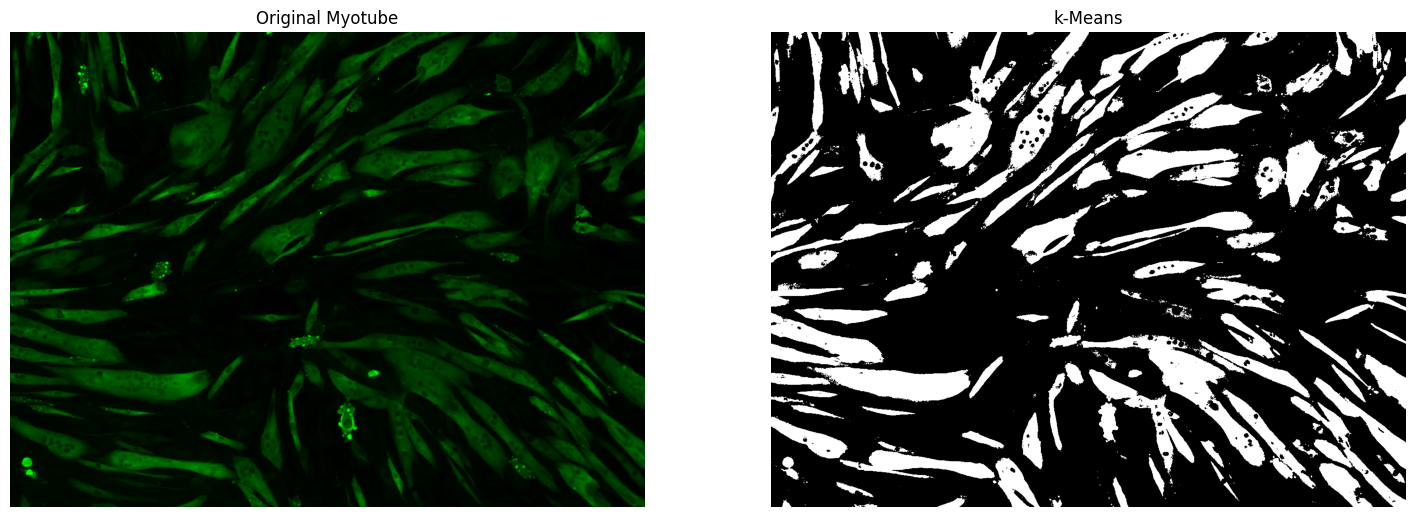
\includegraphics[width=\textwidth]{"images/km_tube.png"}
	\caption[k-Means applied to myotubes]{Foreground detection of myotubes using k-Means}
	\label{figkmtube}
\end{figure}
\begin{figure}
	\centering
	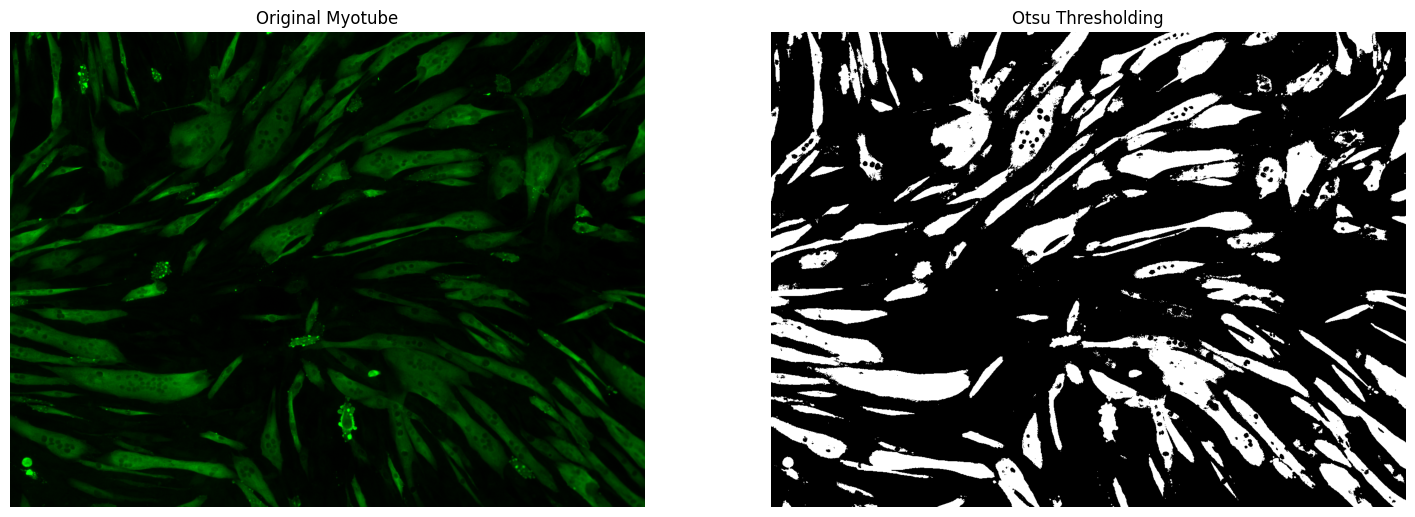
\includegraphics[width=\textwidth]{"images/otsu_tube.png"}
	\caption[Otsu thresholding applied to myotubes]{Foreground detection of myotubes using Otsu thresholding}
	\label{figotsutube}
\end{figure}
\newpage
\subsection{Edge Detection}
As a further attempt to obtain instances of the cells, Canny edge detection \cite{canny} was employed in the hopes that overlapping instances have clear enough borders to be individually identified. In the Canny edge detection algorithm, a Gaussian filter is applied to the image to smooth out any noise present in the image. Next, the intensity gradients of the image are computed highlighting regions of significant change in intensity. The gradient thereby serves as a proxy for the edges. In this case, the Sobel filter \cite{Gonzalez1992} was used to estimate the image gradient. To further refine the edge detection, lower bound cut-off suppression is employed to thin out edges and retain only strong, relevant ones. This is accomplished by iterating over all non-zero pixels in the gradient image and checking whether its a local minimum among its eight neighbors. Following this, a double thresholding technique is utilized to classify pixels as potential edge pixels or non-edge pixels based on their gradient magnitudes. The lower value defines a hard cut-off such that every gradient pixel below that value is set to zero. Any pixel value greater than the larger value defines a strong edge. If a pixel is between the chosen values, the pixel is assumed to part of a weak edge. Weak edges are only kept if they are connected to strong ones. This is also known as hysteresis thresholding. This multi-step process ensures robust edge detection, particularly in scenarios where noise levels vary or edges are fragmented.
\begin{figure}
	\centering
	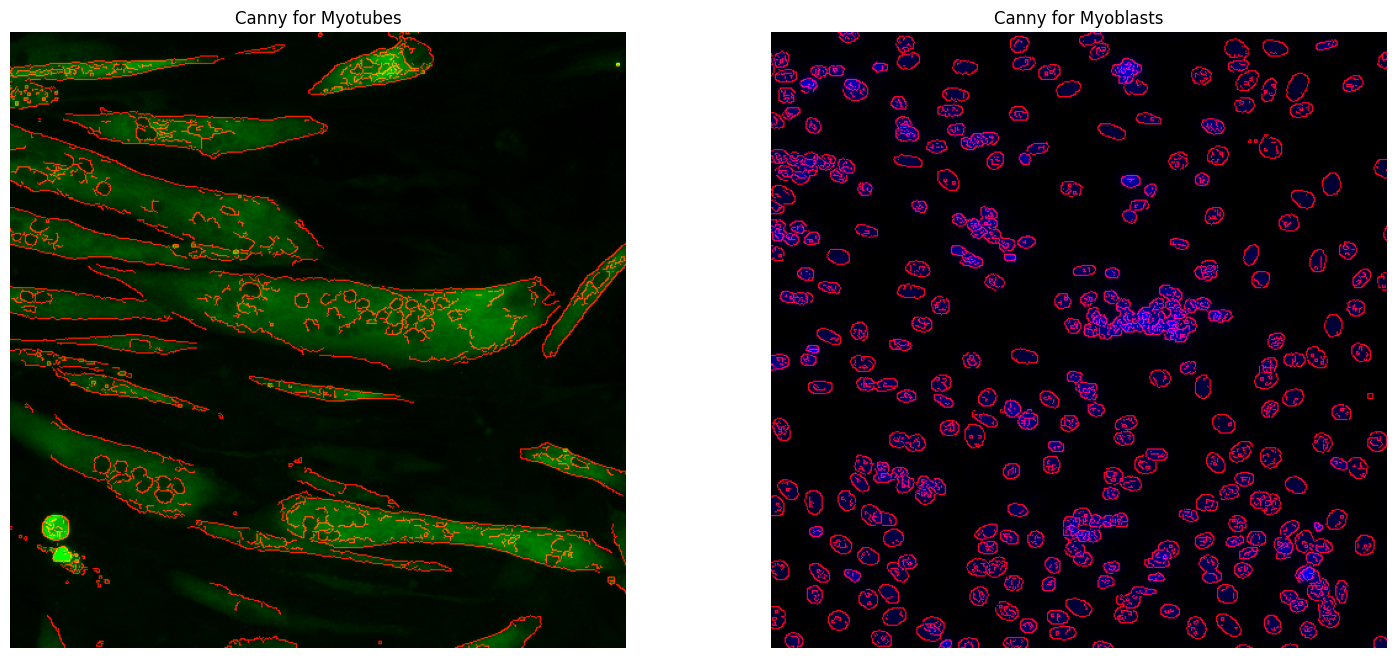
\includegraphics[width=\textwidth]{"images/canny.png"}
	\caption{Canny edge detection applied to both microscopy images.}
	\label{figcanny}
\end{figure}

But yet again, this approach is not particularly desirable because obtaining decent segmentations from it requires a lot of tuning of hyperparameters as well as preprocessing and postprocessing steps tailored to every indivdual image (in addition to running the Canny algorithm in and of itself). Furthermore, the Canny algorithm in and of itself has many tunable parameters and also possesses the downsides that come with thresholding.
\newpage
\subsection{Watershed}
Little math is necessary to understand how segmentation using watersheds functions. First, the image needs to be transformed to grayscale because the resulting single channel needs to be thought of as the a third dimension defining a height profile or topography. In case of a uint8 encoding, the height may take values between 0 and 255. Each pixel can be either of the three following types: a (regional) minimum, a catchment basin or watershed of that minimum, or watershed lines. The first type of pixel is self-explainatory. Continuing with the metaphor, a pixel of second or third type can be thought of in the following manner: picture the position and intensity of the pixel as defining the starting point on the 3d topography defined by the grayscale image. Placing a drop of water on this location can either have it run down (second type) or stay put (third type). All the points where water would run downhill are known as watersheds. All the other points that are not minima define crests, which are the divide (or watershed) lines, beyond which water would not move at all. Iterating over possible intensities starting from the lowest one in the image, or, by analogy, flooding the 3d landscape by poking a hole in the minimum, defines connected areas, or collections of water within a basin, around every regional minimum. Continued flooding will have the water level rise until the first two connected areas merge into one. To prevent that, a dam, whose locations define the pixels of the watershed lines, would need to be built. How to properly construct such dams by means of morphological operations \cite{serra} is thoroughly explained in \cite{Gonzalez1992, coupriewatershed}. The resulting watershed lines are then interpreted as the boundaries of an instance. In this case, a marker-based approach to watershed \cite{meyer} was opted for. Therein, before applying the watershed algorithm, the identification of markers, which are typically connected patches of pixels that represent objects of interest. These markers determine where the flooding begins. 

Based on this intuition, two observations can be made. Firstly, on first glance a catchment basin can have the shape of a myotube or cell nuclei making watershed a sensible segmentation method. Secondly, this method requires the instances to have low grayscale values. This implies that images need to be processed before applying the watershed algorithm since cells are accumulations of high intensity areas. The most naive approach would be a simple inversion of the image. But this can lead to oversegmentation due to noisy sections. More sophisticated approaches either are based on image gradients or a distance transform applied to a binary representation of the original image. The former approach is used in this report and will be its result we be shown before long.

Just from these theoretical discussions alone, it becomes evident that the algorithm will have a hard time differentiating between merging nuclei because they presumably will be interpreted as one single catchment basin due to their intesities being similar. Therefore it still is very difficult to resolve sizable overlaps, unless of course the markers are set such that the algorithm knows that they are different a priori. So again, the results will, again, heavily rely on the quality of preprocessing which is unique work for every new image and something that is ideally avoided. All of these problems are glaringly obvious when applied to the the typical images in Fig.~\ref{figwatershed}.

\begin{figure}
	\centering
	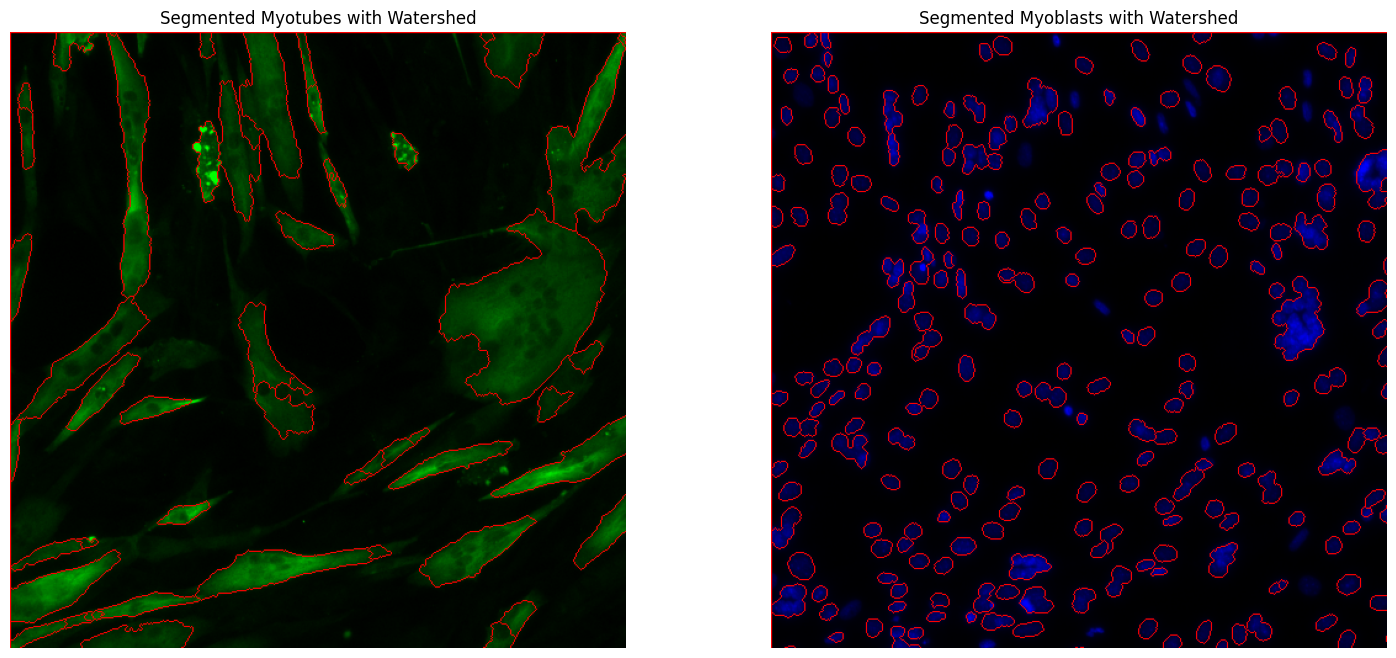
\includegraphics[width=\textwidth]{"images/watershed.png"}
	\caption[Application of watershed]{Marker-based watershed applied to both microscopy images.}
	\label{figwatershed}
\end{figure}

\newpage
\subsection{Ellipse Fitting}
As a last resort for unsupervised methods, it was attempted to fit ellipses to the myoblast images. It is evident that this approach would not work for myotubes due to their oftentimes crooked shapes. But for a typical myoblast image, it does seem to be a sensible approximation. There are several methods that have attempted similar in the literature \cite{panagiotakis2020region, panagiotakis2018cell, kothari2009automated}. All of them have a common structure. The image is preprocessed, which usually consists of methods previously delineated in this section like thresholding, Gaussian filtering, edge detection but also other things like hole-filling. At this point, the typical foreground detection has been performed. At this point, methods start diverging. In some cases ellipses are fit based on the curvature of the foreground. In other cases, many ellipses are fit and the fit with the highest goodness measure like AIC is kept. In addition to that, there are some computed quantities determining whether a segment is large, small, circular, or bright enough to be a cell. All in all, the final part distinguishes touching and overlapping cells one way or another. But even with all these things considered, the segmentation quality is easily influenced by the chosen preprocessing, as can be seen in Fig.~\ref{figellipsefitting}. 
\begin{figure}
	\centering
	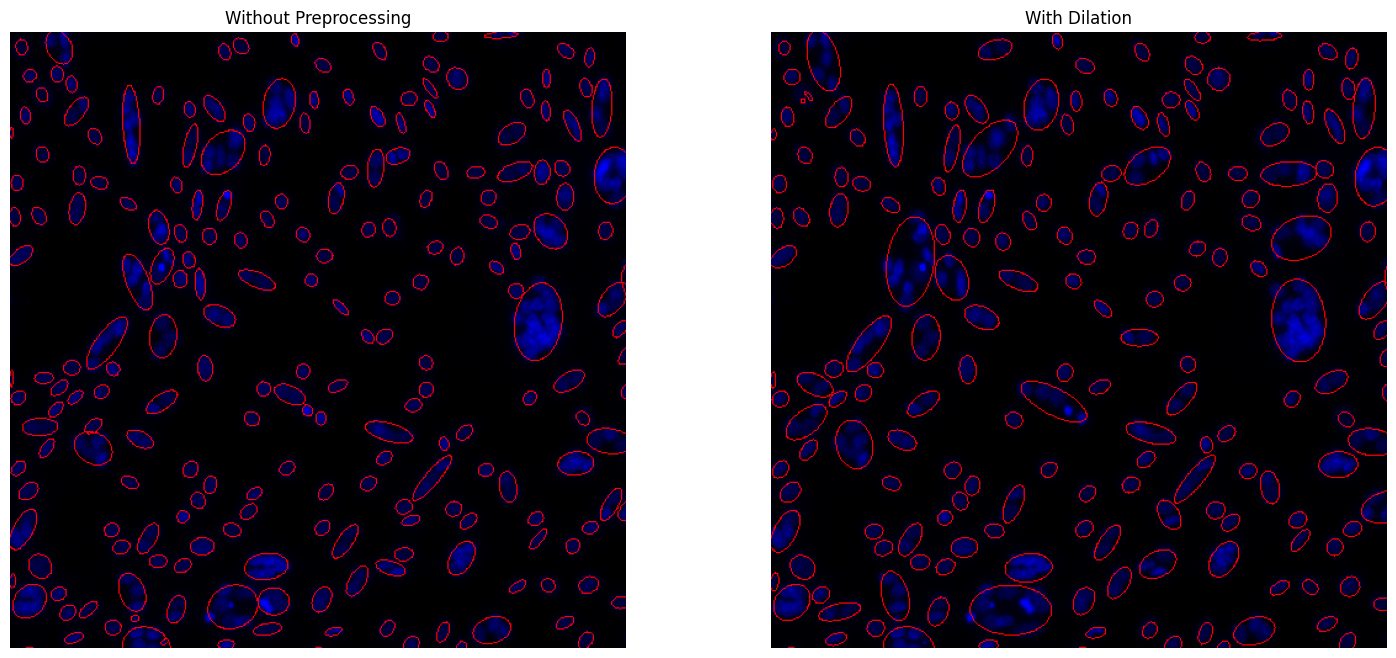
\includegraphics[width=\textwidth]{"images/ellipsefitting.png"}
	\caption[Ellipse Fitting as segmentation]{Ellipse fitting for myoblasts. One additional application of a dilation operation significantly alters the outcome of the segmentation.}
	\label{figellipsefitting}
\end{figure}
